\begin{frame}[fragile]{What is this course?}

\begin{columns}[T,onlytextwidth]
    \begin{column}{0.35\linewidth}
        \begin{figure}
            \centering
            \resizebox{!}{0.5\textheight}{%
            \begin{tikzpicture}
                \node[minimum size=1cm, draw=black, fill=julia_red, circle] (s) {\textcolor{white}{$s_t$}};
                \node[minimum size=1cm, draw=black, fill=julia_red, circle, right=1cm of s] (s2) {\textcolor{white}{$s_{t+1}$}};
                \node[minimum size=1cm, draw=black, fill=julia_purple, circle, below=0.25cm of s] (o) {\textcolor{white}{$o_t$}};
                \node[minimum size=1.3cm, draw=black, fill=julia_green, diamond, above=0.25cm of s] (r) {\textcolor{white}{$r_t$}};
                \node[minimum size=1cm, draw=black, fill=julia_blue, rectangle, above=0.25cm of r] (a) {\textcolor{white}{$a_t$}};
                \node[minimum size=1cm, draw=black, fill=julia_blue, rectangle, left=1cm of a] (am1) {\textcolor{white}{$a_{t-1}$}};
                \node[minimum size=1.3cm, draw=lightgray, fill=julia_green!40, diamond] (rm1) at (am1|-r) {\textcolor{white}{$r_{t-1}$}};
                \node[minimum size=1cm,   draw=lightgray, fill=julia_red!40, circle]  (sm1) at (am1|-s) {\textcolor{white}{$s_{t-1}$}};
                \node[minimum size=1cm,   draw=lightgray, fill=julia_purple!40, circle]  (om1) at (am1|-o) {\textcolor{white}{$o_{t-1}$}};
                \node[minimum size=1cm,   draw=lightgray, fill=julia_blue!40, rectangle] (ap1) at (s2|-a) {\textcolor{white}{$a_{t+1}$}};
                \node[minimum size=1.3cm, draw=lightgray, fill=julia_green!40, diamond]   (rp1) at (s2|-r) {\textcolor{white}{$r_{t+1}$}};
                \node[minimum size=1cm,   draw=lightgray, fill=julia_purple!40, circle]    (op1) at (s2|-o) {\textcolor{white}{$o_{t+1}$}};
                \draw[->] (s) -- (o);
                \draw[->] (s) -- (s2);
                \draw[->] (s) -- (r);
                \draw[->] (a) -- (r);
                \draw[->] (a) [out=0,in=135] to (s2);
                \draw[->] (am1) [out=0,in=135] to (o);
            \end{tikzpicture}}
            \caption{
                \label{fig:pomdps_logo}
                POMDP Sequence.
            }
        \end{figure}
    \end{column}
    \begin{column}{0.65\linewidth}
        {\footnotesize
        \begin{itemize}
            \item A peek into the \texttt{POMDPs.jl} ecosystem of \textbf{\large{\julialogo}} packages
            \item ``But what \textit{are} POMDPs?''
            \begin{itemize}
                \item POMDPs are a \textit{problem formulation} that enable optimal\footnotemark{} sequential decisions to be made in uncertain environments.
            \end{itemize}
            \item Teaching \textit{by example} using interactive \texttt{Pluto.jl} notebooks
            \begin{itemize}
                \item No prior knowledge of MDPs/POMDPs necessary---all are welcome!
            \end{itemize}
        \end{itemize}
        }
    \end{column}
\end{columns}
\footnotetext[1]{or \textit{approximately} optimal.}
\end{frame}

%-------------------------------------------------

\begin{frame}[fragile]{Topics covered in this course}

\begin{highlightblock}
All topics highlight packages that adhere to the \texttt{POMDPs.jl} interface.
\end{highlightblock}

\begin{itemize}
    \item \textbf{Sequential Decision Making}
    \begin{itemize}
        \item \textit{Markov decision processes} (MDPs)
        \item \textit{Partially observable Markov decision processes} (POMDPs)
    \end{itemize}
    \item \textbf{Solution Methods}: Algorithms to solve MDPs/POMDPs
    \begin{itemize}
        \item \textit{Online} and \textit{offline} solvers
        \item \textit{Value function approximation}
    \end{itemize}
    \item \textbf{Simulations}
    \item \textbf{State Estimation using Particle Filters}
    \item \textbf{Reinforcement Learning}
    \item \textbf{Deep Reinforcement Learning}
    \item \textbf{Imitation Learning}
    \item \textbf{Black-Box Validation}
\end{itemize}

\begin{tikzpicture}[remember picture, overlay]
    \node[xshift=-2.8cm, yshift=2.3cm] (img1) at (current page.south east) {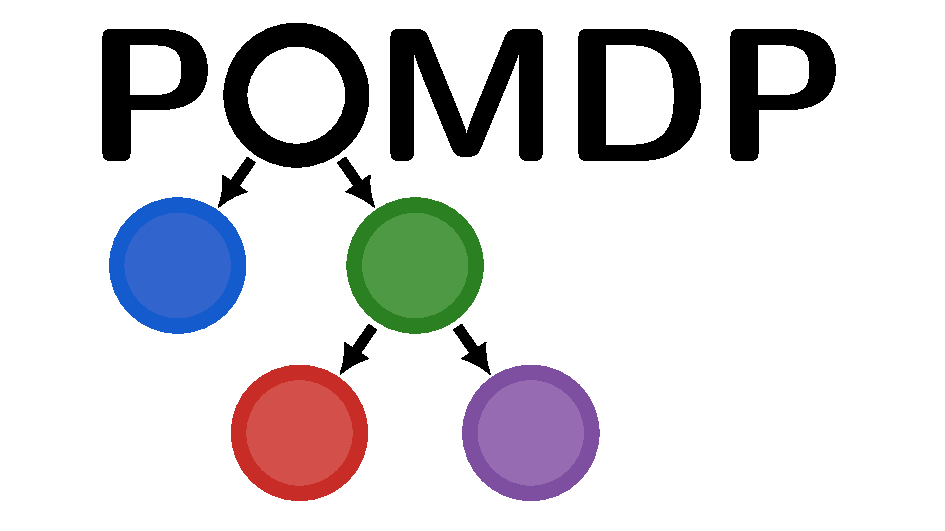
\includegraphics[height=3cm]{images/pomdps_logo.pdf}};
    % \node[xshift=-2cm, yshift=2cm] (img1) at (current page.south east) {\transduration<0-21>{0}\multiinclude[<+->][format=png, graphics={width=\textwidth}]{images/grid-world-animation/gridworld_value_iteration_γ}};
\end{tikzpicture}

\end{frame}

%-------------------------------------------------

\begin{frame}[fragile]{Example problems covered in this course}

Common problems in the literature are used as running examples.

% TODO: Photos.

{\footnotesize
\begin{itemize}
    \item \textbf{$^\text{(MDP)}$ Grid World}: Agent moving around a grid world, looking for rewards.
    \item \textbf{$^\text{(POMDP)}$ Crying Baby}: When to feed a baby, based on crying observations.
    \item \textbf{$^\text{(MDP)}$ 1D Random Walk}: Agent moves around the number line.
    \item \textbf{$^\text{(POMDP)}$ 2D Random Walk}: Estimating state of a moving agent based on observations.
    \item \textbf{$^\text{(MDP)}$ Mountain Car}: Reach a goal up a hill, starting in a valley.
    \item \textbf{$^\text{(MDP)}$ Swinging Pendulum}: Balance a swinging pendulum upright.
\end{itemize}
}

\begin{minipage}[b]{0.18\textwidth}
    \centering
    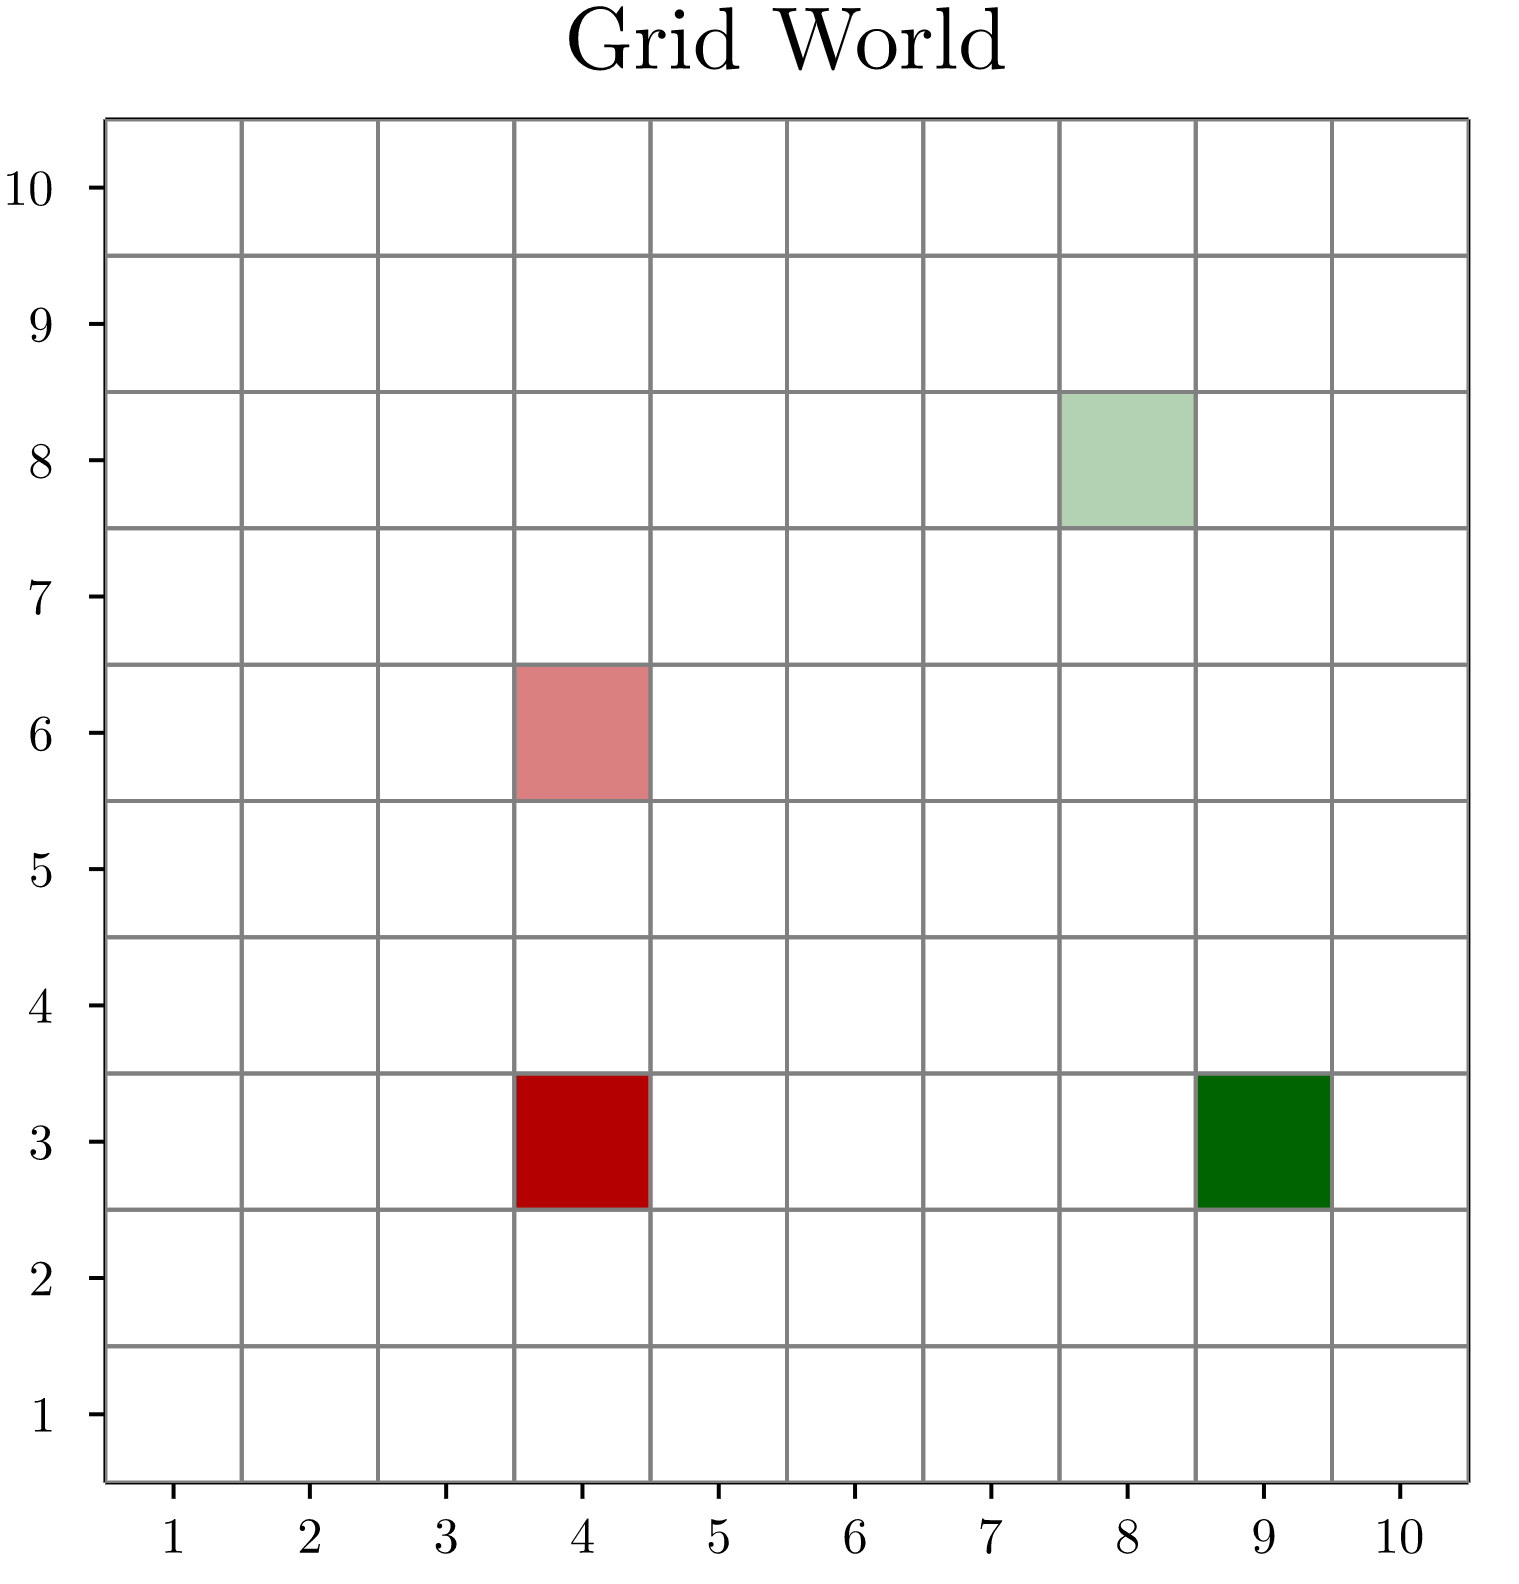
\includegraphics[align=c, width=0.8\textwidth]{images/grid-world.png}
\end{minipage}
\hfill
\begin{minipage}[b]{0.18\textwidth}
    \centering
    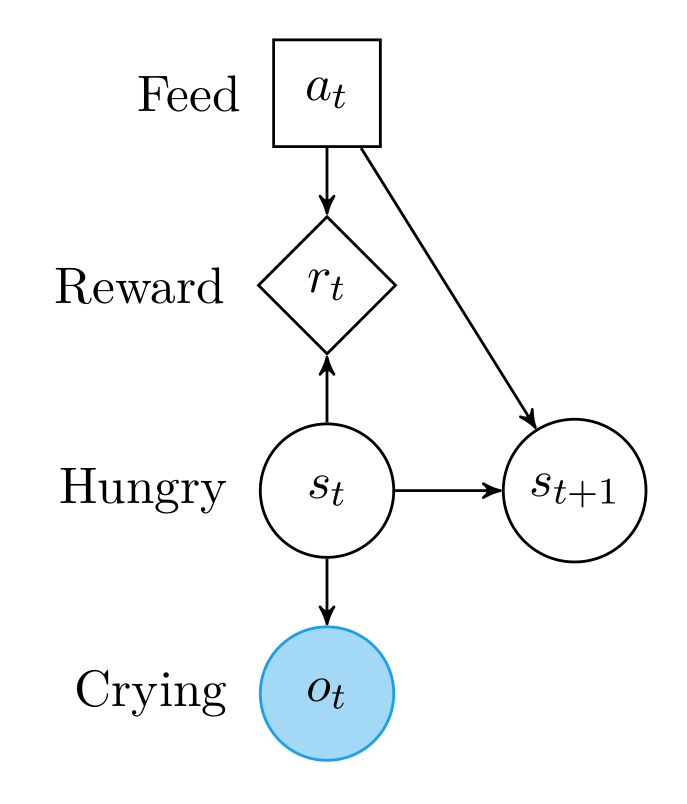
\includegraphics[align=c, width=0.9\textwidth]{images/crying-baby.png}
    % \resizebox{!}{0.3\textheight}{%
    % \begin{tikzpicture}
    %     \node[minimum size=1cm, draw=black, fill=white, circle] (s) {$s_t$};
    %     \node[minimum size=1cm, draw=black, fill=white, circle, right=0.8cm of s] (s2) {$s_{t+1}$};
    %     \node[minimum size=1cm, draw=pastelBlue, fill=pastelBlue!40, circle, below=0.5cm of s] (o) {$o_t$};
    %     \node[minimum size=1cm, draw=black, fill=white, diamond, above=0.5cm of s] (r) {$r_t$};
    %     \node[minimum size=0.8cm, draw=black, fill=white, rectangle, above=0.5cm of r] (a) {$a_t$};
    %     \node[left=0.1 of a, anchor=east] {Feed};
    %     \node[left=0.1 of r, anchor=east] {Reward};
    %     \node[left=0.1 of s, anchor=east] {Hungry};
    %     \node[left=0.1 of o, anchor=east] {Crying};
    %     \draw[->] (s) -- (o);
    %     \draw[->] (s) -- (s2);
    %     \draw[->] (s) -- (r);
    %     \draw[->] (a) -- (r);
    %     \draw[->] (a) -- (s2);
    % \end{tikzpicture}}
\end{minipage}
\hfill
\begin{minipage}[b]{0.18\textwidth}
    \centering
    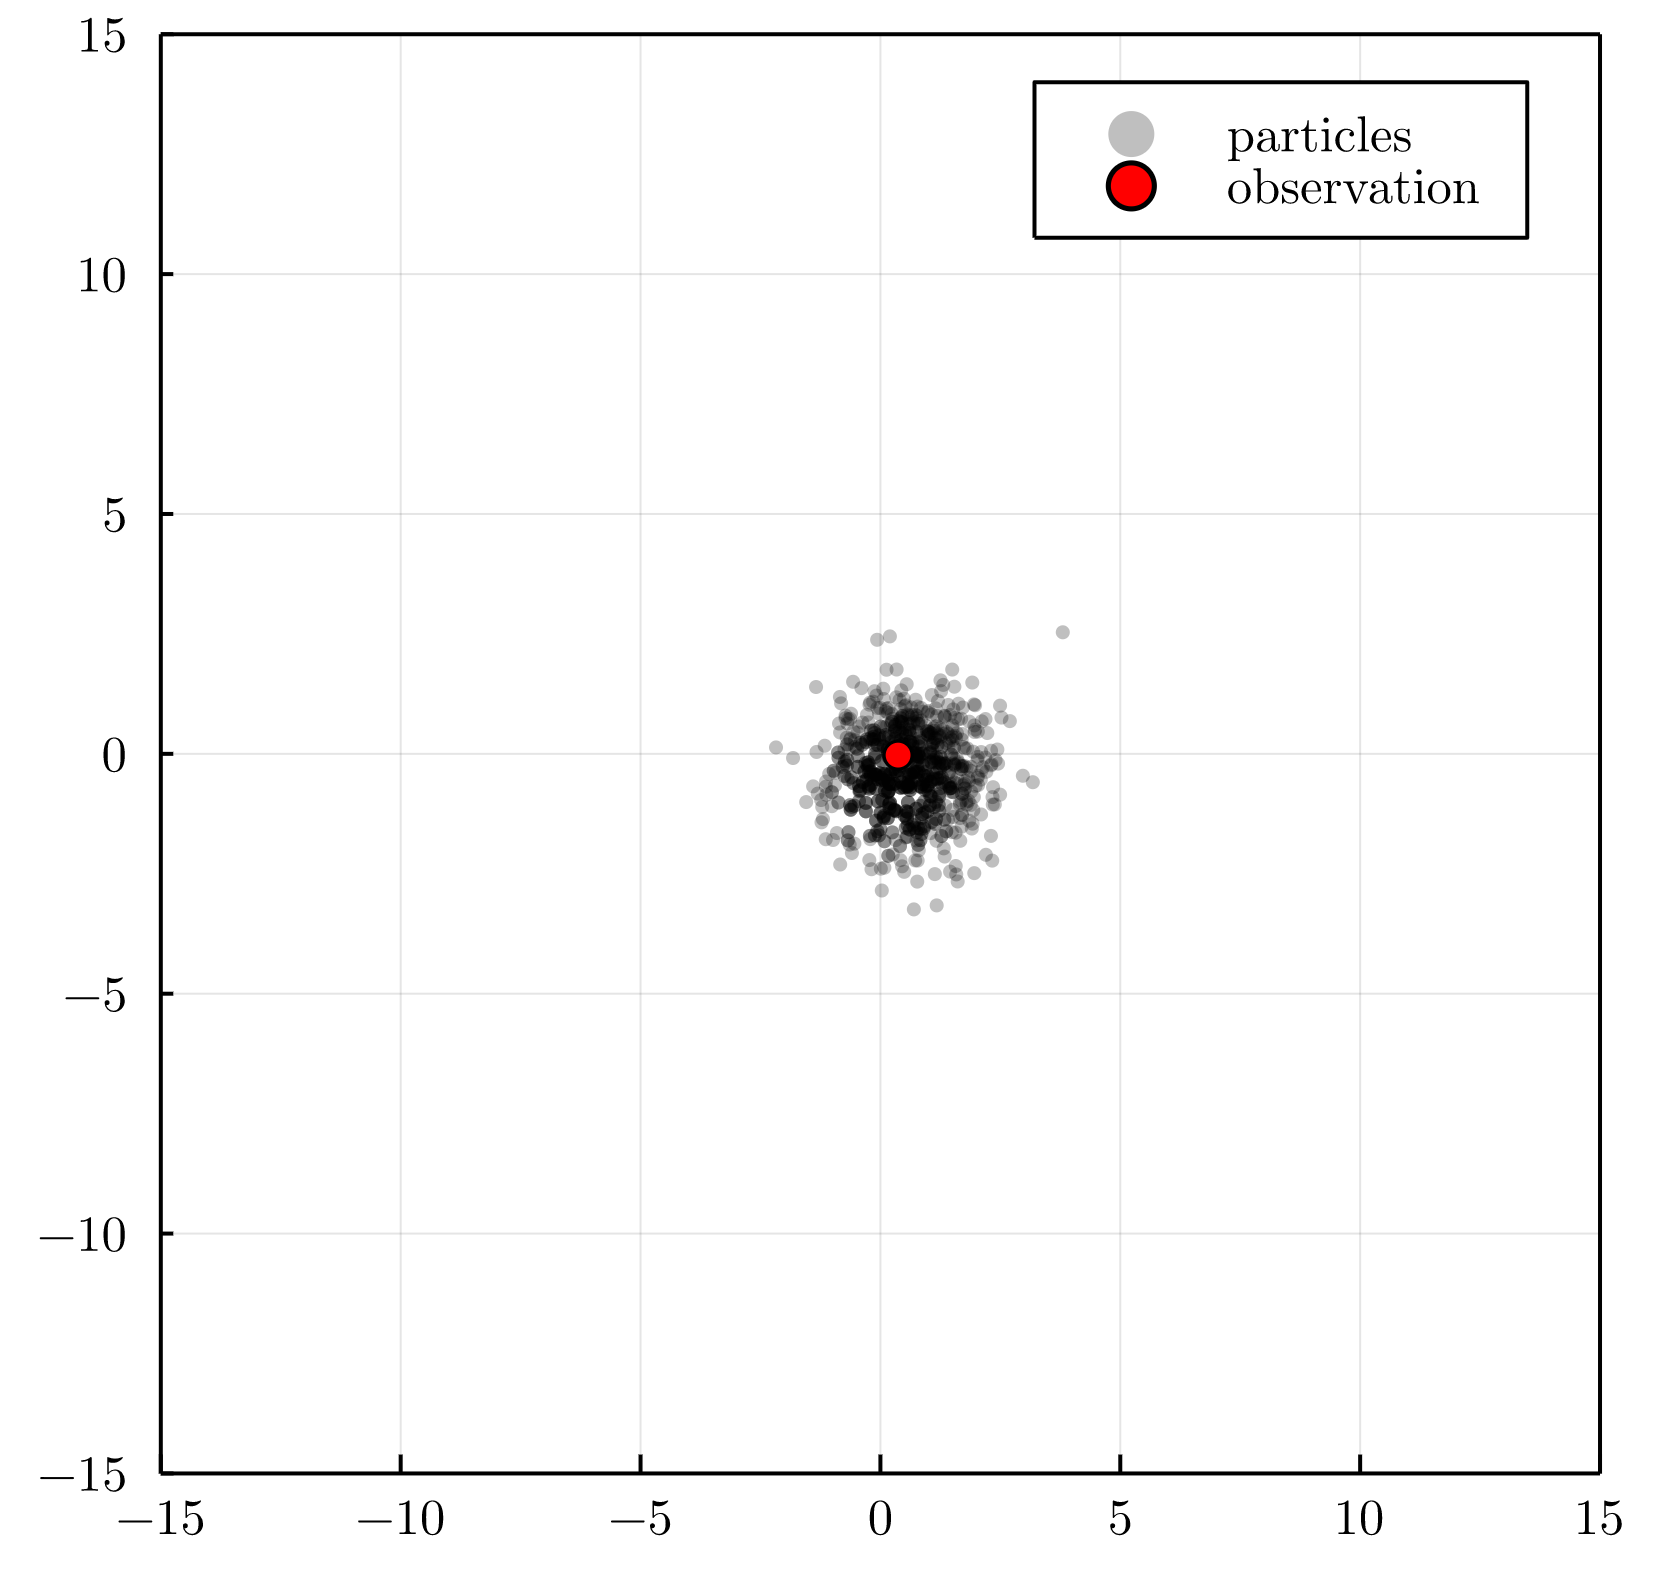
\includegraphics[align=c, width=1.0\textwidth]{images/particle-filter.png}
\end{minipage}
\hfill
\begin{minipage}[b]{0.18\textwidth}
    \centering
    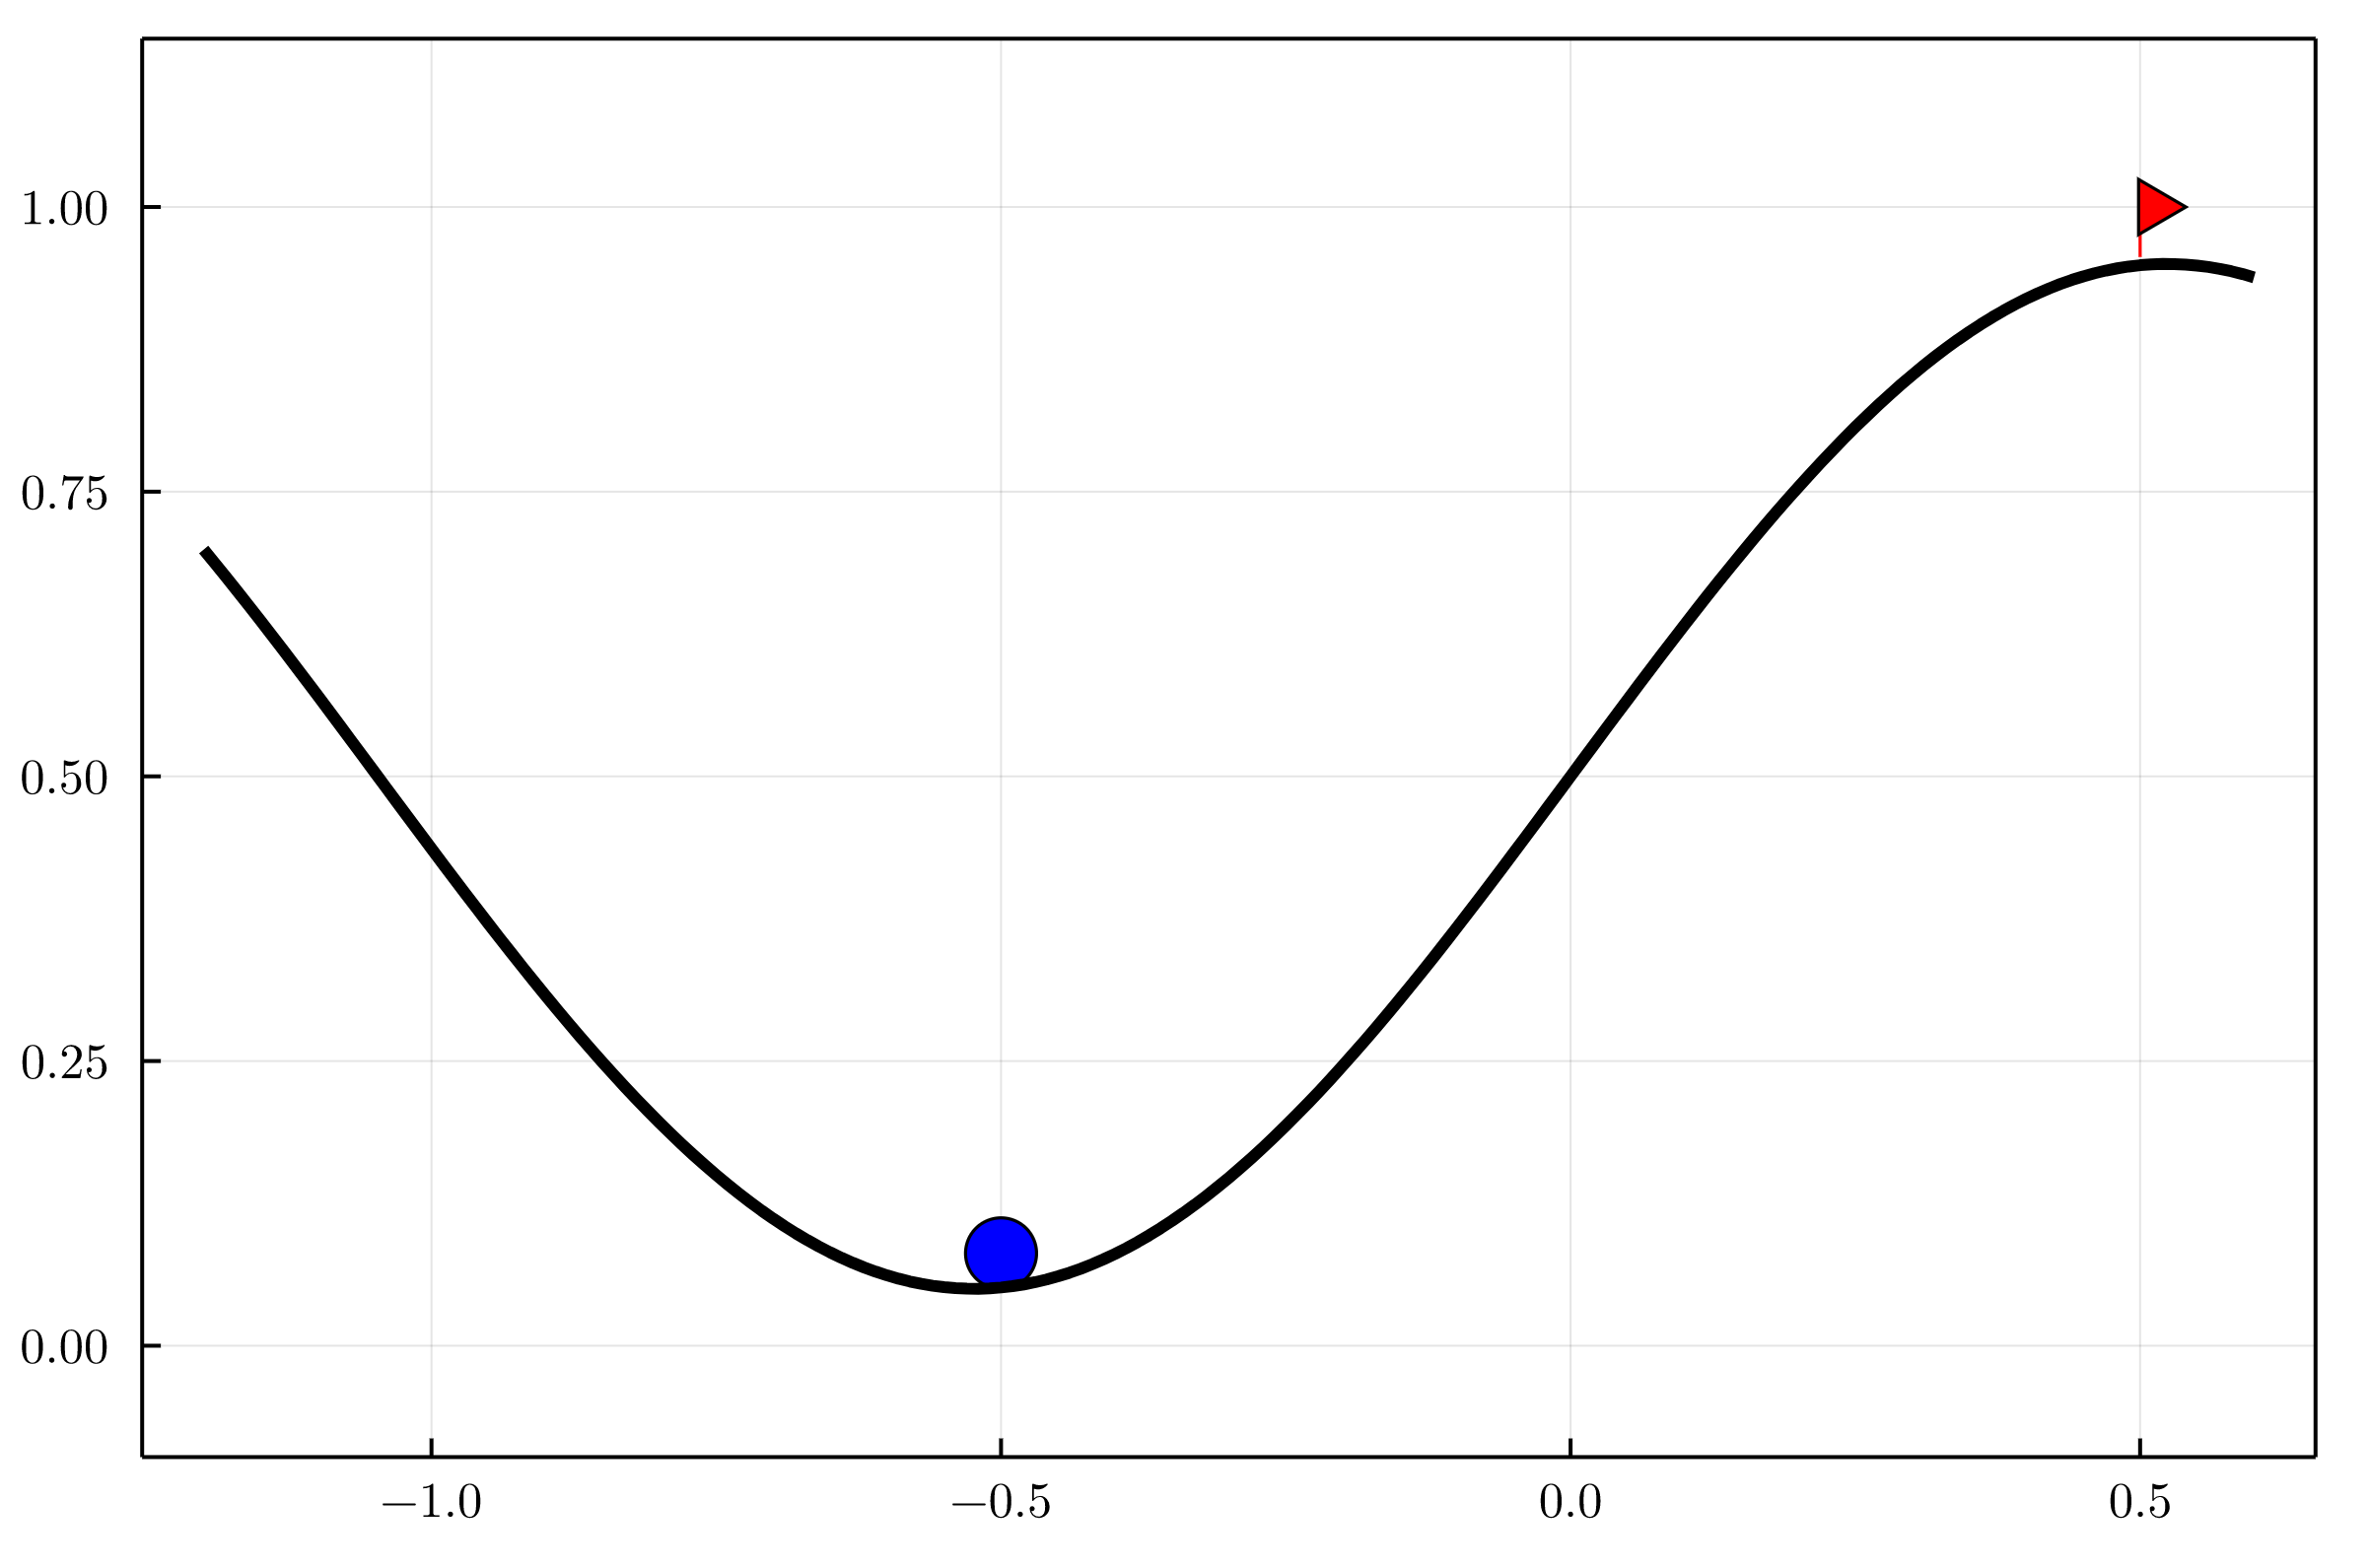
\includegraphics[align=c, width=1.0\textwidth]{images/mountain-car.png}
\end{minipage}
\hfill
\begin{minipage}[b]{0.18\textwidth}
    \centering
    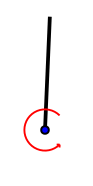
\includegraphics[align=c, width=0.5\textwidth]{images/pendulum.png}
\end{minipage}

\end{frame}

%-------------------------------------------------

\begin{frame}[fragile]{\texttt{POMDPs.jl} package ecosystem}

\begin{highlightblock}
The \texttt{POMDPs.jl} package itself contains the interface to define problem definitions.
\end{highlightblock}

\phantom{}

Other packages provide supporting tools that contain most of the functionality:

\begin{columns}[T,onlytextwidth]
    \begin{column}{0.24\linewidth}
        {\scriptsize
        \begin{itemize}
            \item {\color{julia_green}\href{https://github.com/JuliaPOMDP/QuickPOMDPs.jl}{\texttt{QuickPOMDPs.jl}}}
            \item {\color{julia_blue}\href{https://github.com/JuliaPOMDP/POMDPModelTools.jl}{\texttt{POMDPModelTools.jl}}}
            \item {\color{julia_red}\href{https://github.com/JuliaPOMDP/POMDPPolicies.jl}{\texttt{POMDPPolicies.jl}}}
            \item {\color{julia_green}\href{https://github.com/JuliaPOMDP/POMDPSimulators.jl}{\texttt{POMDPSimulators.jl}}}
            \item {\color{julia_purple}\href{https://github.com/JuliaPOMDP/POMDPModels.jl}{\texttt{POMDPModels.jl}}}
            \item {\color{julia_blue}\href{https://github.com/JuliaPOMDP/POMDPGallery.jl}{\texttt{POMDPGallery.jl}}}
            \item {\color{julia_red}\href{https://github.com/JuliaPOMDP/BeliefUpdaters.jl}{\texttt{BeliefUpdaters.jl}}}
            \item {\color{julia_green}\href{https://github.com/JuliaPOMDP/ParticleFilters.jl}{\texttt{ParticleFilters.jl}}}
        \end{itemize}
        }
    \end{column}
    \begin{column}{0.40\linewidth}
        {\scriptsize
        \begin{itemize}
            \item {\color{julia_blue}\href{https://github.com/JuliaPOMDP/DiscreteValueIteration.jl}{\texttt{DiscreteValueIteration.jl}}}
            \item {\color{julia_red}\href{https://github.com/JuliaPOMDP/LocalApproximationValueIteration.jl}{\texttt{LocalApproximationValueIteration.jl}}}
            \item {\color{julia_green}\href{https://github.com/JuliaPOMDP/GlobalApproximationValueIteration.jl}{\texttt{GlobalApproximationValueIteration.jl}}}
            \item {\color{julia_purple}\href{https://github.com/JuliaPOMDP/MCTS.jl}{\texttt{MCTS.jl}}}
            \item {\color{julia_blue}\href{https://github.com/JuliaPOMDP/TabularTDLearning.jl}{\texttt{TabularTDLearning.jl}}}
            \item {\color{julia_red}\href{https://github.com/JuliaPOMDP/DeepQLearning.jl}{\texttt{DeepQLearning.jl}}}
            \item {\color{julia_green}\href{https://github.com/ancorso/Crux.jl}{\texttt{Crux.jl}}}
            \item {\color{julia_purple}\href{https://github.com/sisl/POMDPStressTesting.jl}{\texttt{POMDPStressTesting.jl}}}
            \item {\color{julia_blue}\href{https://github.com/JuliaPOMDP/DiscreteValueIteration.jl}{\texttt{QMDP.jl}}}
            \item {\color{julia_red}\href{https://github.com/JuliaPOMDP/LocalApproximationValueIteration.jl}{\texttt{FIB.jl}}}
        \end{itemize}
        }
    \end{column}
    \begin{column}{0.32\linewidth}
        {\scriptsize
        \begin{itemize}
            \item {\color{julia_green}\href{https://github.com/JuliaPOMDP/GlobalApproximationValueIteration.jl}{\texttt{BeliefGridValueIteration.jl}}}
            \item {\color{julia_purple}\href{https://github.com/JuliaPOMDP/MCTS.jl}{\texttt{SARSOP.jl}}}
            \item {\color{julia_blue}\href{https://github.com/JuliaPOMDP/TabularTDLearning.jl}{\texttt{BasicPOMCP.jl}}}
            \item {\color{julia_red}\href{https://github.com/JuliaPOMDP/DeepQLearning.jl}{\texttt{ARDESPOT.jl}}}
            \item {\color{julia_green}\href{https://github.com/JuliaPOMDP/Crux.jl}{\texttt{MCVI.jl}}}
            \item {\color{julia_purple}\href{https://github.com/JuliaPOMDP/POMDPStressTesting.jl}{\texttt{POMDPSolve.jl}}}
            \item {\color{julia_blue}\href{https://github.com/JuliaPOMDP/TabularTDLearning.jl}{\texttt{IncrementalPruning.jl}}}
            \item {\color{julia_red}\href{https://github.com/JuliaPOMDP/DeepQLearning.jl}{\texttt{POMCPOW.jl}}}
            \item {\color{julia_green}\href{https://github.com/JuliaPOMDP/Crux.jl}{\texttt{AEMS.jl}}}
            \item {\color{julia_purple}\href{https://github.com/JuliaPOMDP/POMDPStressTesting.jl}{\texttt{PointBasedValueIteration.jl}}}
        \end{itemize}
        }
    \end{column}
\end{columns}

\end{frame}

%-------------------------------------------------

\begin{frame}[fragile]{Other resources}

There are many \textit{excellent} resources on MDPs/POMDPs and reinforcement learning:

{\scriptsize
\begin{itemize}
    \item \textbf{Introduction to Reinforcement Learning with David Silver} ({\color{julia_blue}\url{https://deepmind.com/learning-resources/-introduction-reinforcement-learning-david-silver}})
    \item \textbf{Sutton \& Barto, \textit{Reinforcement Learning: An Introduction}} ({\color{julia_blue}\url{http://incompleteideas.net/book/the-book.html}})
    \item \textbf{Kochenderfer, Wheeler, \& Wray, \textit{Algorithms for Decision Making}} ({\color{julia_blue}\url{https://algorithmsbook.com/}})
    \item \textbf{Egorov, Sunberg, et al., \textit{POMDPs.jl: A Framework for Sequential Decision Making under Uncertainty
}, Journal of Machine Learning Research, 2017} ({\color{julia_blue}\url{https://www.jmlr.org/papers/volume18/16-300/16-300.pdf}})
\end{itemize}
}

\end{frame}

%-------------------------------------------------

%-------------------------------------------------

\begin{frame}[plain,c]{}

\begin{center}
\LARGE \textsc{MDPs: Markov Decision Processes}
\textcolor[RGB]{100,100,100}{\rule{\linewidth}{0.2pt}}

{\color{cardinal}\textbf{\Large{J}\normalsize{ULIA} \Large{A}\normalsize{CADEMY}: \Large{POMDP}\normalsize{S.JL}}}\\
{\normalsize\textsc{Decision Making Under Uncertainty}}

\end{center}

\end{frame}

%-------------------------------------------------

\begin{frame}[fragile]{What is an MDP?}

\begin{definitionblock}{MDP}
    A \textit{Markov decision process} (MDP) is a \textit{problem formulation} that defines how an agent takes sequential \textit{actions} from \textit{states} in its environment, guided by \textit{rewards}---using uncertainty in how it \textit{transitions} from state to state.
\end{definitionblock}

\phantom{}

\begin{itemize}
    \item Formally, an MDP is defined by the following:
\end{itemize}
\begin{table}[!t]
    {\scriptsize
    \centering
    \caption{\label{tab:solutions} MDP Problem Formulation: $\langle \mathcal{S},\, \mathcal{A},\, T,\, R,\, \gamma \rangle$}
    % \rowcolors{2}{gray!15}{white}
    \begin{threeparttable}
    \begin{tabular}{lll}
        \toprule
        \textbf{Variable} & \textbf{Description} & \textbf{\texttt{POMDPs} Interface} \\
        \midrule
        $\mathcal{S}$ & State space & \texttt{POMDPs.states} \\
        $\mathcal{A}$ & Action space & \texttt{POMDPs.actions} \\
        $T(s^\prime \mid s,a)$ & Transition function & \texttt{POMDPs.transition} \\
        $R(s,a)$ & Reward function & \texttt{POMDPs.reward} \\
        $\gamma \in [0,1]$ & Discount factor & \texttt{POMDPs.discount} \\
        \bottomrule
    \end{tabular}
    \end{threeparttable}
    }
\end{table}

\begin{importantblock}
    {\tiny
    \begin{center}
    Remember, an MDP is a \textit{\textbf{problem formulation}} and \textit{\textbf{not an algorithm}}.
  
    An MDP formulation enables the use of solution methods, i.e. algorithms.
    \end{center}
    }
\end{importantblock}

\end{frame}

%-------------------------------------------------

\begin{frame}[fragile]{MDP Example: Grid World}

\begin{highlightblock}
    In the \textbf{Grid World} problem, an \textit{agent} moves around a grid attempting to collect as much reward ({\color{julia_green}\textbf{green cells}}) as possible, avoiding negative rewards ({\color{julia_red}\textbf{red cells}}).
\end{highlightblock}

\begin{figure}
    \centering
    \def\svgwidth{\columnwidth}
    \scalebox{0.6}{\input{images/grid-world-states.pdf_tex}}
\end{figure}

\begin{tikzpicture}[remember picture, overlay]
    \node[xshift=-6.18cm, yshift=4.05cm, minimum size=0.2cm, inner sep=0pt, outer sep=0pt, draw=black, fill=yellow, circle] (agent-base) at (current page.south east) {};
    \node[xshift=-2.8cm, yshift=2.3cm, text width=5cm, align=center] (agent-label) at (current page.south east) {Agent's current position\\(i.e., state)};
    \draw[->, dashed] (agent-base) -- (agent-label);
\end{tikzpicture}

\end{frame}

%-------------------------------------------------

\begin{frame}[fragile]{MDP: State space}

\begin{definitionblock}{State space $\mathcal{S}$}

    A set of all possible \textbf{\textit{states}} an agent can be in (discrete or continuous).
\end{definitionblock}

\begin{figure}
    \centering
    \def\svgwidth{\columnwidth}
    \scalebox{0.6}{\input{images/grid-world-states.pdf_tex}}
\end{figure}

\begin{tikzpicture}[remember picture, overlay]
    \node[xshift=3.0cm, yshift=4.0cm, text width=4.2cm, align=center] (state-desc) at (current page.south west) {\textbf{Grid World example}:\\All possible $(x,y)$ cells in a $10\times10$ grid\\(i.e., 100 discrete states)};

    \node[xshift=-6.18cm, yshift=4.05cm, minimum size=0.2cm, inner sep=0pt, outer sep=0pt, draw=black, fill=yellow, circle] (state-base) at (current page.south east) {};
    \node[xshift=-3.2cm, yshift=2.3cm, text width=4cm, align=center] (state-label) at (current page.south east) {\textbf{State}\\$(x,y)$ of $(9,7)$};
    \draw[->, dashed] (state-base) -- (state-label);
\end{tikzpicture}

\end{frame}

%-------------------------------------------------

\begin{frame}[fragile]{MDP: Action space}

\begin{definitionblock}{Action space $\mathcal{A}$}

    A set of all possible \textbf{\textit{actions}} an agent can take (discrete or continuous).
\end{definitionblock}

\begin{figure}
    \hspace{1cm}
    \centering
    \def\svgwidth{\columnwidth}
    \scalebox{0.6}{\input{images/grid-world-actions.pdf_tex}}
\end{figure}

\begin{tikzpicture}[remember picture, overlay]
    \node[xshift=3.0cm, yshift=4.0cm, text width=5cm, align=center] (action-desc) at (current page.south west) {\textbf{Grid World example}:\\The four (discrete) cardinal directions:\\$[\texttt{up}, \texttt{down}, \texttt{left}, \texttt{right}]$};

    \node[xshift=-5.55cm, yshift=2.7cm, minimum size=0.1cm, inner sep=0pt, outer sep=0pt, draw=black, fill=black, circle] (action-base) at (current page.south east) {};
    \node[xshift=-2.5cm, yshift=2.3cm, text width=3cm, align=center] (action-label) at (current page.south east) {Take action \texttt{down} in state $(9,4)$};
    \draw[->, dashed] (action-base) -- (action-label);
\end{tikzpicture}

\end{frame}

%-------------------------------------------------

\begin{frame}[fragile]{MDP: Transition function}

{\scriptsize
\begin{definitionblock}{Transition function\footnotemark[1] $T(s^\prime \mid s, a)$}

    Defines how the agent \textbf{\textit{transitions}} from the current state $s$ to the next state $s^\prime$ when taking action $a$.

    Returns a \textit{\textbf{probability distribution}} over all possible next states $s^\prime$ given $(s,a)$.
\end{definitionblock}
}

\begin{figure}
    \hspace{9.5cm}
    \centering
    \begin{tikzpicture}    
        \draw[step=1cm,gray,very thin] (0,0) grid (3,3);

        \filldraw[fill=julia_blue!70, draw=gray, very thin] (1,2) rectangle (2,3);
        \node[] at (1.5,2.5) {\scriptsize$0.7$};

        \filldraw[fill=julia_blue!10, draw=gray, very thin] (0,1) rectangle (1,2);
        \node[] at (0.5,1.5) {\scriptsize$0.1$};

        \filldraw[fill=julia_blue!10, draw=gray, very thin] (1,0) rectangle (2,1);
        \node[] at (1.5,0.5) {\scriptsize$0.1$};

        \filldraw[fill=julia_blue!10, draw=gray, very thin] (2,1) rectangle (3,2);
        \node[] at (2.5,1.5) {\scriptsize$0.1$};

        \filldraw[fill=white, draw=black] (1,1) rectangle (2,2);
        \node[] at (1.5,1.6) {$\uparrow$};
        \node[] at (1.5,1.3) {$a$};
        \node[] at (1.15,1.85) {\color{gray}$s$};
    \end{tikzpicture}
\end{figure}

\begin{tikzpicture}[remember picture, overlay]
    \node[xshift=6.0cm, yshift=3.5cm, text width=15cm, align=center, font=\footnotesize] (action-desc) at (current page.south west) {\textbf{Grid World example}:\\Stochastic transitions (incorporates randomness/uncertainty).
    \\Action $a{\;=\;}\texttt{up}$ from state $s$.
    \\{\color{julia_blue}70\% chance of transitioning correctly.}
    \\{\color{julia_blue!70}30\% chance (${10\%\times3}$) of transitioning incorrectly.\footnotemark[2]{}}};
\end{tikzpicture}

\footnotetext[1]{Sometimes called the \textit{transition model}.}
\footnotetext[2]{i.e., a different action is taken.}

\end{frame}

%-------------------------------------------------

\begin{frame}[fragile]{MDP: Reward function}

\begin{definitionblock}{Reward function\footnotemark[1]{} $R(s,a)$}

    A defines the \textbf{\textit{reward}} an agent receives when taking action $a$ from state $s$.
\end{definitionblock}

\begin{figure}
    \hspace{5cm}
    \centering
    \def\svgwidth{\columnwidth}
    \scalebox{0.6}{\input{images/grid-world-rewards.pdf_tex}}
    \vspace{-1cm} % NOTE: footnote placement hack
\end{figure}

\begin{tikzpicture}[remember picture, overlay]
    \node[xshift=4.0cm, yshift=3.5cm, text width=8cm, align=center, font=\footnotesize] (action-desc) at (current page.south west) {\textbf{Grid World example}:\\Two cells contain {\color{julia_green}\textbf{positive rewards}}\\and two cells contain {\color{julia_red}\textbf{negative rewards}},\\all others are {\color{black!80}\textbf{zero}}.};
\end{tikzpicture}

\footnotetext[1]{Sometimes called the \textit{reward model}.}

\end{frame}

%-------------------------------------------------

\begin{frame}[fragile]{MDP: Discount factor}

{\scriptsize
\begin{definitionblock}{Discount factor $\gamma \in [0,1]$}

    \item The \textbf{\textit{discount factor}} controls how myopic (short-sighted) the agent is in its decision making (e.g., when $\gamma=0$, the agent only cares about immediate rewards (myopic) and as $\gamma \to 1$, the agent takes in potential future information in its decision making process).
\end{definitionblock}
}

\phantom{}

\captionsetup[sub]{font=tiny, justification=centering}
% NOTE: added [,trim=1cm 0 1cm 0,clip] to the \includegraphics call in the *.pdf_tex files.

\begin{figure}
    \begin{subfigure}[b]{0.24\textwidth}
        \def\svgwidth{\columnwidth}
        \input{images/grid-world-gamma-0.pdf_tex}
        \caption{Short-sighted\\(no reward spread)}
    \end{subfigure}
    \begin{subfigure}[b]{0.24\textwidth}
        \def\svgwidth{\columnwidth}
        \input{images/grid-world-gamma-0.5.pdf_tex}
        \caption{Some future\\reward\footnotemark[1] is spread}
    \end{subfigure}
    \begin{subfigure}[b]{0.24\textwidth}
        \def\svgwidth{\columnwidth}
        \input{images/grid-world-gamma-0.95.pdf_tex}
        \caption{Future reward\\is nicely spread}
    \end{subfigure}
    \begin{subfigure}[b]{0.24\textwidth}
        \def\svgwidth{\columnwidth}
        \input{images/grid-world-gamma-1.0.pdf_tex}
        \caption{Dominated by\\the future reward}
    \end{subfigure}
\end{figure}

\footnotetext[1]{The sum of the \textit{discounted future rewards} is called the \textit{utility} $U(s)$ or the \textit{value} $V(s)$ of a state.}

\end{frame}

%-------------------------------------------------

\begin{frame}[fragile]{\texttt{QuickPOMDPs}: Grid World}

\begin{lrbox}{\gridworldcode}%
\begin{lstlisting}[language=JuliaLocal, style=julia]
using POMDPs, POMDPModelTools, QuickPOMDPs

struct State; x::Int; y::Int end # State definition
@enum Action UP DOWN LEFT RIGHT # Action definition

𝒮 = [[State(x,y) for x=1:10, y=1:10]..., State(-1,-1)] # State-space
𝒜 = [UP, DOWN, LEFT, RIGHT] # Action-space

const MOVEMENTS = Dict(UP=>State(0,1), DOWN=>State(0,-1), LEFT=>State(-1,0), RIGHT=>State(1,0))
Base.:+(s1::State, s2::State) = State(s1.x + s2.x, s1.y + s2.y) # Helper for applying actions

function T(s, a) # Transition function
    R(s) != 0 && return Deterministic(State(-1,-1))
    Nₐ = length(𝒜)
    next_states = Vector{State}(undef, Nₐ + 1)
    probabilities = zeros(Nₐ + 1)
    for (i, a′) in enumerate(𝒜)
        prob = (a′ == a) ? 0.7 : (1 - 0.7) / (Nₐ - 1)
        destination = s + MOVEMENTS[a′]
        next_states[i+1] = destination
        if 1 ≤ destination.x ≤ 10 && 1 ≤ destination.y ≤ 10
            probabilities[i+1] += prob
        end
    end    
    (next_states[1], probabilities[1]) = (s, 1 - sum(probabilities))
    return SparseCat(next_states, probabilities)
end

function R(s, a=missing) # Reward function
    if s == State(4,3)
        return -10
    elseif s == State(4,6)
        return -5
    elseif s == State(9,3)
        return 10
    elseif s == State(8,8)
        return 3
    end
    return 0
end

abstract type GridWorld <: MDP{State, Action} end

mdp = QuickMDP(GridWorld,
    states     = 𝒮,
    actions    = 𝒜,
    transition = T,
    reward     = R,
    discount   = 0.95,
    isterminal = s->s==State(-1,-1));
\end{lstlisting}
\end{lrbox}%



\begin{columns}[T,onlytextwidth]
    \begin{column}{0.43\linewidth}
        % print the listing box.
        \scalebox{0.28}{\usebox{\gridworldcode}}
    \end{column}
    \begin{column}{0.57\linewidth}
        {\footnotesize
        \begin{itemize}
            \item This code$^a$ defines the entire \textit{Grid World} problem using \texttt{QuickPOMDPs.jl}
            \begin{itemize}
                \item Just a sneak-peek: we'll walk through this in detail in the \texttt{Pluto} notebooks
            \end{itemize}
        \end{itemize}
        }
        \begin{figure}
            % \hspace{5cm}
            \centering
            \def\svgwidth{\columnwidth}
            \scalebox{0.7}{\input{images/grid-world-rewards-title.pdf_tex}}
        \end{figure}
        \footnotetext[1]{Yes, this is self-contained---copy and paste it into a notebook or REPL!}
    \end{column}
\end{columns}


\end{frame}

%-------------------------------------------------

\begin{frame}{MDP solvers}

A number of ways to solve MDPs are implemented in the following packages.

\begin{table}[!t]
    {\scriptsize
    \centering
    \caption{\label{tab:solutions} MDP Solution Methods}
    \rowcolors{2}{white}{gray!15}
    \begin{threeparttable}
    \begin{tabular}{lccc}
        \toprule
        % \textbf{Package} & \textbf{Online/Offline} & \textbf{Continuous States} & \textbf{Continuous Actions}\\
        \textbf{Package} & \textbf{Online/Offline} & \textbf{State Spaces} & \textbf{Actions Spaces}\\
        \midrule
        \href{https://github.com/JuliaPOMDP/DiscreteValueIteration.jl}{\texttt{DiscreteValueIteration.jl}} & Offline & Discrete & Discrete \\
        \href{https://github.com/JuliaPOMDP/LocalApproximationValueIteration.jl}{\texttt{LocalApproximationValueIteration.jl}} & Offline & Continuous & Discrete \\
        \href{https://github.com/JuliaPOMDP/GlobalApproximationValueIteration.jl}{\texttt{GlobalApproximationValueIteration.jl}} & Offline & Continuous & Discrete \\
        \href{https://github.com/JuliaPOMDP/MCTS.jl}{\texttt{MCTS.jl}}\tnote{*} & Online & Continuous & Continuous \\
        \bottomrule
    \end{tabular}
    \begin{tablenotes}
        \scriptsize
        \item[*] {Monte Carlo Tree Search.}
    \end{tablenotes}
    \end{threeparttable}
    }
\end{table}

{\tiny
\begin{importantblock}
When defining your problem, the \textbf{\textit{type}} of state and action space is very important!
\end{importantblock}
}

\end{frame}

%-------------------------------------------------

\begin{frame}{Reinforcement learning solvers}

{\small Certain problems are better suited in the \textit{reinforcement learning} (RL) domain. Several RL solvers that adhere to the \texttt{POMDPs.jl} interface are implemented in the following packages.}

\begin{table}[!t]
    {\tiny
    \centering
    \caption{\label{tab:solutions} Reinforcement Learning Solution Methods}
    \rowcolors{2}{white}{gray!15}
    \begin{threeparttable}
    \begin{tabular}{lccp{0.5\linewidth}}
        \toprule
        \textbf{Package} & \textbf{State Spaces} & \textbf{Actions Spaces} & \textbf{Algorithms Implemented} \\
        \midrule
        \href{https://github.com/JuliaPOMDP/TabularTDLearning.jl}{\texttt{TabularTDLearning.jl}} & Discrete & Discrete & Q-learning, SARSA, SARSA-$\lambda$ \\
        \href{https://github.com/JuliaPOMDP/DeepQLearning.jl}{\texttt{DeepQLearning.jl}} & Continuous & Discrete & DQN, Double DQN, Dueling DQN, Recurrent Q-learning\\
        \href{https://github.com/ancorso/Crux.jl}{\texttt{Crux.jl}} & Continuous & Continuous & DQN, REINFORCE, PPO, A2C, DDPG, TD3, SAC, Behavior Cloning, GAIL, AdVIL, AdRIL, SQIL, ASAF\\
        \bottomrule
    \end{tabular}
    % \begin{tablenotes}
    %     \tiny
    %     \item[*] {Monte Carlo Tree Search.}
    % \end{tablenotes}
    \end{threeparttable}
    }
\end{table}

{\tiny
\begin{importantblock}
When defining your problem, the \textbf{\textit{type}} of state, action, and observation space is very important!
\end{importantblock}
}

\end{frame}

%-------------------------------------------------


%-------------------------------------------------

%-------------------------------------------------

\begin{frame}[fragile]{What is a POMDP?}

\begin{definitionblock}{POMDP}
    A \textit{Partially observable Markov decision process} (POMDP) is an MDP with \textit{state uncertainty}---meaning we cannot know the \textit{true} state, only a \textit{belief} about the true state using \textit{observations}.
\end{definitionblock}

\phantom{}

\begin{itemize}
    \item Formally, a POMDP is defined by the following:
\end{itemize}
\begin{table}[!t]
    {\scriptsize
    \centering
    \caption{\label{tab:solutions} MDP Problem Formulation: $\langle \mathcal{S},\, \mathcal{A},\, {\color{darkblue}\mathcal{O}},\, T,\, R,\, {\color{darkblue}O},\, \gamma \rangle$}
    % \rowcolors{2}{gray!15}{white}
    \begin{threeparttable}
    \begin{tabular}{lll}
        \toprule
        \textbf{Variable} & \textbf{Description} & \textbf{\texttt{POMDPs} Interface} \\
        \midrule
        $\mathcal{S}$ & State space & \texttt{POMDPs.states} \\
        $\mathcal{A}$ & Action space & \texttt{POMDPs.actions} \\
        $\mathcal{O}$ & Observation space & \texttt{POMDPs.observations} \\
        $T(s^\prime \mid s,a)$ & Transition function & \texttt{POMDPs.transition} \\
        $R(s,a)$ & Reward function & \texttt{POMDPs.reward} \\
        $O(o \mid s^\prime)$ & Observation function & \texttt{POMDPs.observation} \\
        $\gamma \in [0,1]$ & Discount factor & \texttt{POMDPs.discount} \\
        \bottomrule
    \end{tabular}
    \end{threeparttable}
    }
\end{table}

\begin{importantblock}
    {\footnotesize
    \begin{center}
    Remember, a POMDP is a \textit{\textbf{problem formulation}} and \textit{\textbf{not an algorithm}}.
  
    A POMDP formulation enables the use of solution methods, i.e. algorithms.
    \end{center}
    }
\end{importantblock}

\end{frame}

%-------------------------------------------------

\begin{frame}[fragile]{Example POMDP: Crying Baby Problem}

\begin{columns}[T,onlytextwidth]
    \begin{column}{0.55\columnwidth}
        \begin{figure}
            \centering
            \begin{tikzpicture}
                \node[minimum size=1cm, draw=black, fill=white, circle] (s) {$s_t$};
                \node[minimum size=1cm, draw=black, fill=white, circle, right=0.8cm of s] (s2) {$s_{t+1}$};
                \node[minimum size=1cm, draw=pastelBlue, fill=pastelBlue!40, circle, below=0.5cm of s] (o) {$o_t$};
                \node[minimum size=1cm, draw=black, fill=white, diamond, above=0.5cm of s] (r) {$r_t$};
                \node[minimum size=0.8cm, draw=black, fill=white, rectangle, above=0.5cm of r] (a) {$a_t$};
                \node[left=0.1 of a, anchor=east] {Feed};
                \node[left=0.1 of r, anchor=east] {Reward};
                \node[left=0.1 of s, anchor=east] {Hungry};
                \node[left=0.1 of o, anchor=east] {Crying};
                \draw[->] (s) -- (o);
                \draw[->] (s) -- (s2);
                \draw[->] (s) -- (r);
                \draw[->] (a) -- (r);
                \draw[->] (a) -- (s2);
            \end{tikzpicture}
            \caption{
                \label{fig:crying_baby_pomdp}
                The crying baby POMDP.
            }
        \end{figure}
    \end{column}
    \begin{column}{0.45\columnwidth}
        \begin{itemize}
            \item A simple POMDP with 2 states, 3 actions, and 2 observations:
            \begin{align*}
                \mathcal{S} &= \{\texttt{hungry},\, \texttt{sated}\}\\
                \mathcal{A} &= \{\texttt{feed},\, \texttt{sing},\, \texttt{ignore}\}\\
                \mathcal{O} &= \{\texttt{crying},\, \texttt{quiet}\}
            \end{align*}
        \end{itemize}
    \end{column}
\end{columns}

\end{frame}

%-------------------------------------------------

\begin{frame}[fragile]{\texttt{QuickPOMDPs}: Crying Baby}

\begin{lrbox}{\cryingbabycode}%
\begin{lstlisting}[language=JuliaLocal, style=julia]
crying_pomdp = QuickPOMDP(
    states       = [hungry, full],  # 𝒮
    actions      = [feed, ignore],  # 𝒜
    observations = [crying, quiet], # 𝒪
    initialstate = [full], # Deterministic
    discount     = 0.9, # γ

    transition = function T(s, a)
        if a == feed
            return SparseCat([hungry, full], [0, 1])
        elseif s == hungry && a == ignore
            return SparseCat([hungry, full], [1, 0])
        elseif s == full && a == ignore
            return SparseCat([hungry, full], [0.1, 0.9])
        end
    end,

    observation = function O(s, a, s′)
        if s′ == hungry
            return SparseCat([crying, quiet], [0.8, 0.2])
        elseif s′ == full
            return SparseCat([crying, quiet], [0.1, 0.9])
        end
    end,
    
    reward = (s,a)->(s == hungry ? -10 : 0) + (a == feed ? -5 : 0)
) 
\end{lstlisting}
\end{lrbox}%

% print the listing box.
\scalebox{0.3}{\usebox{\cryingbabycode}}

\end{frame}

%-------------------------------------------------

\begin{frame}{POMDP solvers}

A number of ways to solve POMDPs are implemented in the following packages.

\begin{table}[!t]
    {\tiny
    \centering
    \caption{\label{tab:solutions} POMDP Solution Methods}
    \rowcolors{2}{white}{gray!15}
    \begin{threeparttable}
    \begin{tabular}{lcccc}
        \toprule
        \textbf{Package} & \textbf{Online/Offline} & \textbf{State Spaces} & \textbf{Actions Spaces} & \textbf{Observation Spaces}\\
        \midrule
        \href{https://github.com/JuliaPOMDP/QMDP.jl}{\texttt{QMDP.jl}} & Offline & Discrete & Discrete & Discrete \\
        \href{https://github.com/JuliaPOMDP/FIB.jl}{\texttt{FIB.jl}} & Offline & Discrete & Discrete & Discrete \\
        \href{https://github.com/JuliaPOMDP/BeliefGridValueIteration.jl}{\texttt{BeliefGridValueIteration.jl}} & Offline & Discrete & Discrete & Discrete \\
        \href{https://github.com/JuliaPOMDP/SARSOP.jl}{\texttt{SARSOP.jl}} & Offline & Discrete & Discrete & Discrete \\
        \href{https://github.com/JuliaPOMDP/BasicPOMCP.jl}{\texttt{BasicPOMCP.jl}} & Online & Continuous & Discrete & Discrete \\
        \href{https://github.com/JuliaPOMDP/ARDESPOT.jl}{\texttt{ARDESPOT.jl}} & Online & Continuous & Discrete & Discrete \\
        \href{https://github.com/JuliaPOMDP/MCVI.jl}{\texttt{MCVI.jl}} & Offline & Continuous & Discrete & Continuous \\
        \href{https://github.com/JuliaPOMDP/POMDPSolve.jl}{\texttt{POMDPSolve.jl}} & Offline & Discrete & Discrete & Discrete \\
        \href{https://github.com/JuliaPOMDP/IncrementalPruning.jl}{\texttt{IncrementalPruning.jl}} & Offline & Discrete & Discrete & Discrete \\
        \href{https://github.com/JuliaPOMDP/POMCPOW.jl}{\texttt{POMCPOW.jl}} & Online & Continuous & Continuous & Continuous \\
        \href{https://github.com/JuliaPOMDP/AEMS.jl}{\texttt{AEMS.jl}} & Online & Discrete & Discrete & Discrete \\
        \href{https://github.com/JuliaPOMDP/PointBasedValueIteration.jl}{\texttt{PointBasedValueIteration.jl}} & Offline & Discrete & Discrete & Discrete \\
        \bottomrule
    \end{tabular}
    \end{threeparttable}
    }
\end{table}

{\footnotesize
\begin{importantblock}
When defining your problem, the \textbf{\textit{type}} of state, action, and observation space is very important!
\end{importantblock}
}

\end{frame}

%-------------------------------------------------


%-------------------------------------------------
